
%% bare_conf.tex
%% V1.4b
%% 2015/08/26
%% by Michael Shell
%% See:
%% http://www.michaelshell.org/
%% for current contact information.
%%
%% This is a skeleton file demonstrating the use of IEEEtran.cls
%% (requires IEEEtran.cls version 1.8b or later) with an IEEE
%% conference paper.
%%
%% Support sites:
%% http://www.michaelshell.org/tex/ieeetran/
%% http://www.ctan.org/pkg/ieeetran
%% and
%% http://www.ieee.org/

%%*************************************************************************
%% Legal Notice:
%% This code is offered as-is without any warranty either expressed or
%% implied; without even the implied warranty of MERCHANTABILITY or
%% FITNESS FOR A PARTICULAR PURPOSE! 
%% User assumes all risk.
%% In no event shall the IEEE or any contributor to this code be liable for
%% any damages or losses, including, but not limited to, incidental,
%% consequential, or any other damages, resulting from the use or misuse
%% of any information contained here.
%%
%% All comments are the opinions of their respective authors and are not
%% necessarily endorsed by the IEEE.
%%
%% This work is distributed under the LaTeX Project Public License (LPPL)
%% ( http://www.latex-project.org/ ) version 1.3, and may be freely used,
%% distributed and modified. A copy of the LPPL, version 1.3, is included
%% in the base LaTeX documentation of all distributions of LaTeX released
%% 2003/12/01 or later.
%% Retain all contribution notices and credits.
%% ** Modified files should be clearly indicated as such, including  **
%% ** renaming them and changing author support contact information. **
%%*************************************************************************


% *** Authors should verify (and, if needed, correct) their LaTeX system  ***
% *** with the testflow diagnostic prior to trusting their LaTeX platform ***
% *** with production work. The IEEE's font choices and paper sizes can   ***
% *** trigger bugs that do not appear when using other class files.       ***                          ***
% The testflow support page is at:
% http://www.michaelshell.org/tex/testflow/



\documentclass[conference]{IEEEtran}
% Some Computer Society conferences also require the compsoc mode option,
% but others use the standard conference format.
%
% If IEEEtran.cls has not been installed into the LaTeX system files,
% manually specify the path to it like:
% \documentclass[conference]{../sty/IEEEtran}





% Some very useful LaTeX packages include:
% (uncomment the ones you want to load)


% *** MISC UTILITY PACKAGES ***
%
%\usepackage{ifpdf}
% Heiko Oberdiek's ifpdf.sty is very useful if you need conditional
% compilation based on whether the output is pdf or dvi.
% usage:
% \ifpdf
%   % pdf code
% \else
%   % dvi code
% \fi
% The latest version of ifpdf.sty can be obtained from:
% http://www.ctan.org/pkg/ifpdf
% Also, note that IEEEtran.cls V1.7 and later provides a builtin
% \ifCLASSINFOpdf conditional that works the same way.
% When switching from latex to pdflatex and vice-versa, the compiler may
% have to be run twice to clear warning/error messages.






% *** CITATION PACKAGES ***
%
%\usepackage{cite}
% cite.sty was written by Donald Arseneau
% V1.6 and later of IEEEtran pre-defines the format of the cite.sty package
% \cite{} output to follow that of the IEEE. Loading the cite package will
% result in citation numbers being automatically sorted and properly
% "compressed/ranged". e.g., [1], [9], [2], [7], [5], [6] without using
% cite.sty will become [1], [2], [5]--[7], [9] using cite.sty. cite.sty's
% \cite will automatically add leading space, if needed. Use cite.sty's
% noadjust option (cite.sty V3.8 and later) if you want to turn this off
% such as if a citation ever needs to be enclosed in parenthesis.
% cite.sty is already installed on most LaTeX systems. Be sure and use
% version 5.0 (2009-03-20) and later if using hyperref.sty.
% The latest version can be obtained at:
% http://www.ctan.org/pkg/cite
% The documentation is contained in the cite.sty file itself.






% *** GRAPHICS RELATED PACKAGES ***
%
\ifCLASSINFOpdf
  \usepackage[pdftex]{graphicx}
  % declare the path(s) where your graphic files are
  \graphicspath{{C:/Users/Gautam/Pictures}}
  % and their extensions so you won't have to specify these with
  % every instance of \includegraphics
  \DeclareGraphicsExtensions{.pdf,.jpeg,.png,.jpg}
\else
  % or other class option (dvipsone, dvipdf, if not using dvips). graphicx
  % will default to the driver specified in the system graphics.cfg if no
  % driver is specified.
   \usepackage[dvips]{graphicx}
  % declare the path(s) where your graphic files are
   \graphicspath{{C:/Users/Gautam/Pictures}}
  % and their extensions so you won't have to specify these with
  % every instance of \includegraphics
   \DeclareGraphicsExtensions{.eps}
\fi
% graphicx was written by David Carlisle and Sebastian Rahtz. It is
% required if you want graphics, photos, etc. graphicx.sty is already
% installed on most LaTeX systems. The latest version and documentation
% can be obtained at: 
% http://www.ctan.org/pkg/graphicx
% Another good source of documentation is "Using Imported Graphics in
% LaTeX2e" by Keith Reckdahl which can be found at:
% http://www.ctan.org/pkg/epslatex
%
% latex, and pdflatex in dvi mode, support graphics in encapsulated
% postscript (.eps) format. pdflatex in pdf mode supports graphics
% in .pdf, .jpeg, .png and .mps (metapost) formats. Users should ensure
% that all non-photo figures use a vector format (.eps, .pdf, .mps) and
% not a bitmapped formats (.jpeg, .png). The IEEE frowns on bitmapped formats
% which can result in "jaggedy"/blurry rendering of lines and letters as
% well as large increases in file sizes.
%
% You can find documentation about the pdfTeX application at:
% http://www.tug.org/applications/pdftex





% *** MATH PACKAGES ***
%
%\usepackage{amsmath}
% A popular package from the American Mathematical Society that provides
% many useful and powerful commands for dealing with mathematics.
%
% Note that the amsmath package sets \interdisplaylinepenalty to 10000
% thus preventing page breaks from occurring within multiline equations. Use:
%\interdisplaylinepenalty=2500
% after loading amsmath to restore such page breaks as IEEEtran.cls normally
% does. amsmath.sty is already installed on most LaTeX systems. The latest
% version and documentation can be obtained at:
% http://www.ctan.org/pkg/amsmath





% *** SPECIALIZED LIST PACKAGES ***
%
%\usepackage{algorithmic}
% algorithmic.sty was written by Peter Williams and Rogerio Brito.
% This package provides an algorithmic environment fo describing algorithms.
% You can use the algorithmic environment in-text or within a figure
% environment to provide for a floating algorithm. Do NOT use the algorithm
% floating environment provided by algorithm.sty (by the same authors) or
% algorithm2e.sty (by Christophe Fiorio) as the IEEE does not use dedicated
% algorithm float types and packages that provide these will not provide
% correct IEEE style captions. The latest version and documentation of
% algorithmic.sty can be obtained at:
% http://www.ctan.org/pkg/algorithms
% Also of interest may be the (relatively newer and more customizable)
% algorithmicx.sty package by Szasz Janos:
% http://www.ctan.org/pkg/algorithmicx


\usepackage{booktabs}

% *** ALIGNMENT PACKAGES ***
%
\usepackage{array}
% Frank Mittelbach's and David Carlisle's array.sty patches and improves
% the standard LaTeX2e array and tabular environments to provide better
% appearance and additional user controls. As the default LaTeX2e table
% generation code is lacking to the point of almost being broken with
% respect to the quality of the end results, all users are strongly
% advised to use an enhanced (at the very least that provided by array.sty)
% set of table tools. array.sty is already installed on most systems. The
% latest version and documentation can be obtained at:
% http://www.ctan.org/pkg/array


% IEEEtran contains the IEEEeqnarray family of commands that can be used to
% generate multiline equations as well as matrices, tables, etc., of high
% quality.




% *** SUBFIGURE PACKAGES ***
\ifCLASSOPTIONcompsoc
  \usepackage[caption=false,font=normalsize,labelfont=sf,textfont=sf]{subfig}
\else
  \usepackage[caption=false,font=footnotesize]{subfig}
\fi
% subfig.sty, written by Steven Douglas Cochran, is the modern replacement
% for subfigure.sty, the latter of which is no longer maintained and is
% incompatible with some LaTeX packages including fixltx2e. However,
% subfig.sty requires and automatically loads Axel Sommerfeldt's caption.sty
% which will override IEEEtran.cls' handling of captions and this will result
% in non-IEEE style figure/table captions. To prevent this problem, be sure
% and invoke subfig.sty's "caption=false" package option (available since
% subfig.sty version 1.3, 2005/06/28) as this is will preserve IEEEtran.cls
% handling of captions.
% Note that the Computer Society format requires a larger sans serif font
% than the serif footnote size font used in traditional IEEE formatting
% and thus the need to invoke different subfig.sty package options depending
% on whether compsoc mode has been enabled.
%
% The latest version and documentation of subfig.sty can be obtained at:
% http://www.ctan.org/pkg/subfig




% *** FLOAT PACKAGES ***
%
%\usepackage{fixltx2e}
% fixltx2e, the successor to the earlier fix2col.sty, was written by
% Frank Mittelbach and David Carlisle. This package corrects a few problems
% in the LaTeX2e kernel, the most notable of which is that in current
% LaTeX2e releases, the ordering of single and double column floats is not
% guaranteed to be preserved. Thus, an unpatched LaTeX2e can allow a
% single column figure to be placed prior to an earlier double column
% figure.
% Be aware that LaTeX2e kernels dated 2015 and later have fixltx2e.sty's
% corrections already built into the system in which case a warning will
% be issued if an attempt is made to load fixltx2e.sty as it is no longer
% needed.
% The latest version and documentation can be found at:
% http://www.ctan.org/pkg/fixltx2e


%\usepackage{stfloats}
% stfloats.sty was written by Sigitas Tolusis. This package gives LaTeX2e
% the ability to do double column floats at the bottom of the page as well
% as the top. (e.g., "\begin{figure*}[!b]" is not normally possible in
% LaTeX2e). It also provides a command:
%\fnbelowfloat
% to enable the placement of footnotes below bottom floats (the standard
% LaTeX2e kernel puts them above bottom floats). This is an invasive package
% which rewrites many portions of the LaTeX2e float routines. It may not work
% with other packages that modify the LaTeX2e float routines. The latest
% version and documentation can be obtained at:
% http://www.ctan.org/pkg/stfloats
% Do not use the stfloats baselinefloat ability as the IEEE does not allow
% \baselineskip to stretch. Authors submitting work to the IEEE should note
% that the IEEE rarely uses double column equations and that authors should try
% to avoid such use. Do not be tempted to use the cuted.sty or midfloat.sty
% packages (also by Sigitas Tolusis) as the IEEE does not format its papers in
% such ways.
% Do not attempt to use stfloats with fixltx2e as they are incompatible.
% Instead, use Morten Hogholm'a dblfloatfix which combines the features
% of both fixltx2e and stfloats:
%
% \usepackage{dblfloatfix}
% The latest version can be found at:
% http://www.ctan.org/pkg/dblfloatfix




% *** PDF, URL AND HYPERLINK PACKAGES ***
%
%\usepackage{url}
% url.sty was written by Donald Arseneau. It provides better support for
% handling and breaking URLs. url.sty is already installed on most LaTeX
% systems. The latest version and documentation can be obtained at:
% http://www.ctan.org/pkg/url
% Basically, \url{my_url_here}.




% *** Do not adjust lengths that control margins, column widths, etc. ***
% *** Do not use packages that alter fonts (such as pslatex).         ***
% There should be no need to do such things with IEEEtran.cls V1.6 and later.
% (Unless specifically asked to do so by the journal or conference you plan
% to submit to, of course. )


% correct bad hyphenation here

 

\begin{document}
%
% paper title
% Titles are generally capitalized except for words such as a, an, and, as,
% at, but, by, for, in, nor, of, on, or, the, to and up, which are usually
% not capitalized unless they are the first or last word of the title.
% Linebreaks \\ can be used within to get better formatting as desired.
% Do not put math or special symbols in the title.
\title{Importance of Cooperative gameplay in Multiplayer online battle arena (MOBA) games}


% author names and affiliations
% use a multiple column layout for up to three different
% affiliations
\author{\IEEEauthorblockN{Gautam Baghel, Magy Seif El-Nasr}
\IEEEauthorblockA{College of Computer and Information Science\\
Northeastern University\\
Boston, Massachusetts 02115\\}

}

% conference papers do not typically use \thanks and this command
% is locked out in conference mode. If really needed, such as for
% the acknowledgment of grants, issue a \IEEEoverridecommandlockouts
% after \documentclass

% for over three affiliations, or if they all won't fit within the width
% of the page, use this alternative format:
% 
%\author{\IEEEauthorblockN{Michael Shell\IEEEauthorrefmark{1},
%Homer Simpson\IEEEauthorrefmark{2},
%James Kirk\IEEEauthorrefmark{3}, 
%Montgomery Scott\IEEEauthorrefmark{3} and
%Eldon Tyrell\IEEEauthorrefmark{4}}
%\IEEEauthorblockA{\IEEEauthorrefmark{1}School of Electrical and Computer Engineering\\
%Georgia Institute of Technology,
%Atlanta, Georgia 30332--0250\\ Email: see http://www.michaelshell.org/contact.html}
%\IEEEauthorblockA{\IEEEauthorrefmark{2}Twentieth Century Fox, Springfield, USA\\
%Email: homer@thesimpsons.com}
%\IEEEauthorblockA{\IEEEauthorrefmark{3}Starfleet Academy, San Francisco, California 96678-2391\\
%Telephone: (800) 555--1212, Fax: (888) 555--1212}
%\IEEEauthorblockA{\IEEEauthorrefmark{4}Tyrell Inc., 123 Replicant Street, Los Angeles, California 90210--4321}}




% use for special paper notices
%\IEEEspecialpapernotice{(Invited Paper)}




% make the title area
\maketitle

% As a general rule, do not put math, special symbols or citations
% in the abstract
\begin{abstract}
Computer game contributes a huge part to modern culture. Among different types of computer games, the multi-player online battle arena games generated an electronic sports community and attracted plentiful audiences. LOL (League of Legends), as one of the leading multi-player online battle arena games, Riot has a big responsibility on analyzing game data and improving game experiences to players. This paper applies classification methods to identify the contribution of teamwork performance and star player performance to winning. Through various methods verification, the results show using teamwork behavior has higher prediction accuracy than using one-star player performance data in a match. In sum, the results with a data set of 534398 team data in 2015 recommend better teamwork contributes more to winning than single star player performance.
\end{abstract}

% no keywords




% For peer review papers, you can put extra information on the cover
% page as needed:
% \ifCLASSOPTIONpeerreview
% \begin{center} \bfseries EDICS Category: 3-BBND \end{center}
% \fi
%
% For peerreview papers, this IEEEtran command inserts a page break and
% creates the second title. It will be ignored for other modes.
\IEEEpeerreviewmaketitle



\section{Introduction}
% no \IEEEPARstart

In recent years, there is a rise in popularity of MOBA (Multi-Player Online Battle Arena) games. These games are usually composed of several players forming teams and competing against each other in matches. Each match can range from few minutes of play to hours of play. League of Legends alone reportedly has over 100 million monthly active users \cite{Loterina}. Professional players have made careers out of playing professional MOBA games with earnings in the range of two million dollars annually \cite{esports}. Electronic sports (eSports) are becoming an important part of our culture. In this paper, we are interested in (a) understanding how teamwork is established within a team and how that may impact win/loss. Understanding if the team is important rather than just one player which means more engagement to all the team rather than them relying upon one has design and user experience implication, but also perhaps a learning implication. For game designers, it may be environmental elements of the game which contribute to synergy in a game. For producers, it may be involvement of more players and getting them hooked on the game. For players, it gives them an opportunity to refine their skills where it proved to be inadequate.

To achieve this goal, the paper uses a game analytics approach where data from a MOBA game is analyzed through machine learning algorithms. There has been similar work in this area. Looking at several aspects of team composition from player personalities to champion types in the game. Player personalities may vary in different players altogether and the findings are preliminary. Champion type analysis only looks at the composition based on champion specific skills, player effectiveness in using the champion is not evident. Team versus star player analysis gives a better picture of cooperation versus competition in the game.  

In order to tackle this problem, we analyzed 534,398 data of team statistics from MOBA game. We used analyzed the team vs. star player on the team in terms of their contribution to winning/losing. To answer that we turned this into a classification question where we predict win/loss based on team features vs. star-player features. This kind of analysis is the first of its kind to understand the contribution of team members and features influencing win/loss from different team members. The contribution is in the results that we found and it adds to previous work on team level analysis in MOBA game from a different perspective. 

This paper is divided into the following section. First, we discuss previous work in more detail outlining the open problems given the work done in MOBA games. Second, we discuss the game we used and the dataset. Third, we discuss the algorithms used and results obtained. We then discuss the results in more detail. We conclude by outlining the contribution and applications of the results.  

 

% You must have at least 2 lines in the paragraph with the drop letter
% (should never be an issue)
%I wish you the best of success.

%\hfill mds
 
%\hfill August 26, 2015




%\subsection{Subsection Heading Here}
%Subsection text here.


%\subsubsection{Subsubsection Heading Here}
%Subsubsection text here.


\section{Previous Work}
A study by Christoph Eggert and team \cite{Eggert2015} which classified players into sets of classes and segments of games with respect to their roles, effectiveness in time (early/late) and support items/ damage types. Using Logistic Regression, Random Forest and Bayesian Networks to reduce the set of player classes for better accuracy in predicting the winner. A team-based approach to MOBA is similar but on aspects divided on roles. Limitations may include predetermining roles in the game which may lead to some early misdirection in team formation.

 Personality aspects have also been taken into consideration while forming a team where the study investigated how personality trait and expertise affect virtual team interactions \cite{Balthazard2004}. Using correlation analysis, regression analysis, and a series of post hoc t-tests they were able to hypothesize the mechanisms through which personal characteristics of individuals are aggregated via group-level dynamics to produce group-level outcomes and approached the  team v/s individual performance based on personality traits. They concluded that the results were preliminary and since they were formed into interdependent teams for only the relatively brief duration of their task it cannot be used universally.

Another team analysis 'Learning Dota 2 Team Compositions' \cite{Agarwala2014}, studied teams using PCA and second order PCA with Logistic regression was done for a different MOBA game Dota 2, using hero composition. They concluded that cleaner data or better models are needed. Factors responsible may have been player skills which were not taken into consideration.

The clustering algorithm used in the paper Player Behavior and Optimal Team Composition based on champion types is done in Online Multiplayer Game study based on champion types by Hao Yi Ong and team \cite{Bainbridge2009} was effective in forming teams based on champion types. The focus in this paper is on player types like ambush-er, magic, physical, support etc. and team composition from that, whether a specific class of champions has any effect on winning. It uses clustering of players based on their behaviors, visualizing the data using PCA and predicting the winner using classification. Factors not taken into consideration was team play behaviors like assists and player skill-based classification.

Research done in similar area  Player Skill Decomposition in Multiplayer Online Battle Arenas \cite{Chen2016} looked at 14 cooperative games to find out game-play design aspects which determine the interaction between player. Their research showed that helping occurred when the game was difficult for players which may be a factor in teams which win in the league of legends. Results may be time dependent and as the game changes rapidly over the years, player strategies may have evolved differently from MOBA games. 

Making use of game log data, 'On Successful Team Formation' \cite{Pobiedina2013b} chose a statistical approach to identify factors that increase the chance of a team to win. Their hypothesis being better role distribution in a team increases the chance to win a game,     teams with more experienced players have a higher chance to win, playing with friends increases the chance to win and
the selection of a proper leader as well as a good matching of heroes inside a team positively influence the success. Using ANOVA test and Mann-Whitney-Wilcoxon-tests they were able to identify better Individual Hero Selection vs Team Hero Selection with log-linear analysis. In this approach, specific Gameplay elements not considered the part of analysis since MOBAs tend to be different from other online multiplayer games where gameplay aspects like inhibitors, dragons are quintessential to form strategies it falls short.
  
Effectiveness of Machine Learning algorithms in predicting game outcome by systematic review and compare performance of most frequently used machine learning algorithms for prediction of the match winner from the teams' drafts in DotA 2 computer game \cite{Semenov} deals with algorithms such as Naive Bayes classifier, Logistic Regression and Decision trees to validate consistency in data mining. Using the algorithms this paper comes up with standard performance metrics for players. This paper deals with different algorithms than the ones previously presented.

\section{Game and Data}
The data set consists of about two million League of Legends (LOL) matches that happened in 2015 summer retrieved using riots API system. The game mode is called 5-vs-5 ranked matches of a solo queue which is extensively played MOBA mode. A typical such match involves ten players who form two teams of five. Each match consists of ten rows with statistics of each player as shown in Fig 1. Star player and team data set are segregated which will consist of two rows per match. In the Star player data set, a player who falls under the category of the star player will be placed on each team and in the team data set aggregate of all the player from each team will make two rows per match.


\begin{figure}[!t]
%\centering
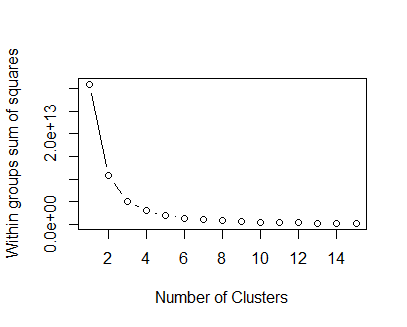
\includegraphics[width=\linewidth]{tab4}
% where an .eps filename suffix will be assumed under latex, 
% and a .pdf suffix will be assumed for pdflatex; or what has been declared
% via \DeclareGraphicsExtensions.
\caption{Dataset with retrieved from riot's API}
\label{fig_sim}
\end{figure}


\section{Feature Extraction}
We derived several features from the given data above: 
\begin{itemize}
  \item \textbf{Star Player}  Using backward feature selection which includes all the predictors and recursively removes the predictors which are less influential, goldEarned was the most important predictor with Akaike information criterion that overrules other predictors. The findings here were corroborated in the heat map of the predictors show that gold earned supersedes every other predictor by huge margins \cite{Patterson}. 
  \item \textbf{Team features}  A similar approach is made as with the star player analysis. Using backward feature selection on assist components of the game which reduces to totalDamageDealt, firstTowerAssist, firstBloodAssist, assists, and firstInhibitorAssist. 
\end{itemize}

\section{Team Features vs. Star Player affecting Win/Loss in Moba Game}


We considered and compared several methods to predict the effect of team vs. star player as features for predicting win/loss. 
After the separation of data set into two distinctive halves, we tried to form a learning model based on the features. The datasets comprised of categorical and quantitative data so every algorithm used had its pros and cons. When choosing reasonable methods, some dimensions are considered. For example, the number of training examples, the feature space dimensionality, the relationship between features, the linearly dependent expiations between features and target variable (winner), the problem of overfitting and the computer system’s capacity on running data analysis. Based on the dimensions we considered, these five models were chosen.

\begin{itemize}
  \item \textbf{Logistic Regression}
We chose this method due to we expect the LOL data features are roughly linear and the hypothesis problem to be linearly separable. This method is also efficient. Also, since LR output can be interpreted as a probability, it is good for predicting winning or losing. 

  \item \textbf{Linear Discriminant Analysis }
Also known as Fisher Linear Discriminant (FLD), is a classical algorithm for pattern recognition. It is an effective feature extraction method. Using this method, the inter-class scatter matrix of the post-projection pattern samples can be maximized, and the intra-class scatter matrix is minimized. In other words, it can guarantee the smallest-in-class distance and the largest inter-class distance in the new space, that is, the pattern can be best separated in that space. However, LDA is not effective when sample information is dependent on variance rather than mean.

  \item \textbf{Quadratic Discriminant Analysis }
LDA requires an assumption of equal variance-covariance matrices between the input variables of the classes. QDA is a modification of LDA which allows for the above heterogeneity of classes' covariance matrices. Since in our team dataset we can't be sure whether the covariance of each of the classes is identical or not it is a good idea to use QDA as well. And it can be used to build the model for more problems. The difference is, when the covariance matrices of different categorical samples are the same, LDA should be chosen. Otherwise, QDA should be used. The reason we use both LDA and QDA is to test which method works better on our problem.

  \item \textbf{Regression Tree}
A Decision Tree (DT) is a graph that uses a branching method to illustrate every possible outcome of a decision. Generally, DT is easier to understand and be explained to most people. Since DT is nonparametric, no worry is needed about whether the data and the outliers are linearly separable. DT’s main drawback is that it is easy to over-fit, which makes the random forest (Random Forest, RF) (or Boosted tree) and other integrated learning algorithm arise. The R package we use is rpart. It solves the over-fitting problem through prune method. It firstly builds a complicated tree model and then estimates the error of each model under different” pruning” conditions according to the Cross-Validation method. This model may prove better as our dataset may contain lots of outliers especially when we analyze the star player. Also, it is useful for our data to be explained in a straightforward way.

  \item \textbf{Clustering}
Another approach is based on unsupervised learning which is different from all the models used above.In clustering we do not train the data set to predict winning, we simply form groups of players with similar characteristics in terms of being a star player or team player. We’ll use our initial training set without segregating it into teams and star players. K-means is a clustering algorithm which tries to form initial cluster centroids and proceeds by repeating cluster assignments and updating centroids. These steps are performed until the algorithm converges. Using the k-means clustering method we’ll append each player a cluster number to which they belong. 
So the dataset currently looks like in Fig. 3.


%----\begin{figure}[!t]
%\centering
%----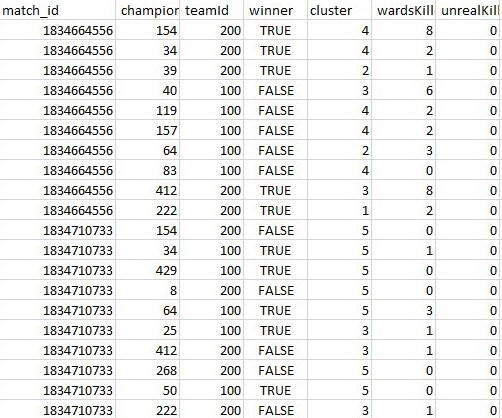
\includegraphics[width=\linewidth]{tab3}
% where an .eps filename suffix will be assumed under latex, 
% and a .pdf suffix will be assumed for pdflatex; or what has been declared
% via \DeclareGraphicsExtensions.
%----\caption{Dataset with a column named cluster included for every player}
%----\label{fig_sim}
%-----\end{figure}


 K-means starts with a random choice of cluster centers and needs the number of clusters to be specified we have to plot and see the number of clusters appropriate for the analysis.

\begin{figure}[!t]
%\centering
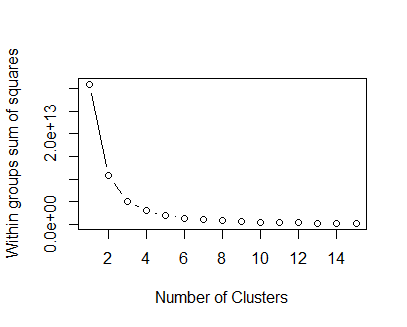
\includegraphics[width=\linewidth]{tab4}
% where an .eps filename suffix will be assumed under latex, 
% and a .pdf suffix will be assumed for pdflatex; or what has been declared
% via \DeclareGraphicsExtensions.
\caption{K-means clustering options}
%\label{fig_sim}
\end{figure}

 From the Fig. 4, five seems to be a good enough cluster choice. At this point, every player in the game will be in a cluster between 1 and 5. For the team analysis now every team will have a score between 5 and 25 by doing the cluster number aggregation. From this number we’ll predict the winner. As the predictors are in higher dimension we’ll use PCA to visualize the data point and which classification method to use. PCA involves all the predictors which constitute to a cooperative gameplay like assists,totalDamageDealt,firstTowerAssist etc. The data points can be seen in Fig. 5.

\begin{figure}[!t]
%\centering
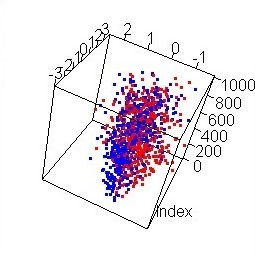
\includegraphics[width=\linewidth]{tab5}
% where an .eps filename suffix will be assumed under latex, 
% and a .pdf suffix will be assumed for pdflatex; or what has been declared
% via \DeclareGraphicsExtensions.
\caption{3D representation of data points using PCA}
%\label{fig_sim}
\end{figure}

 From Fig 5, it seems like data points can be separated through a plane, which provokes the idea of using a support vector machine (SVM). SVM has high classification accuracy and has a good theoretical guarantee to over-fitting. Through selecting appropriate kernel function, it can function well even when facing problems that are not linearly separable. Since SVM is good for highly dimensional space data too, it may prove to be a good choice for prediction.

\end{itemize}

\section{Results}

The validation of results is done using 10-fold cross validation method which divides the dataset into 10 subsets, and the holdout method is repeated 10 times. Each time, one of the 10 subsets is used as the test set and the other 9 subsets are put together to form a training set. Then the average error across all 10 trials is computed. The advantage of this method is that it matters less how the data gets divided. Every data point gets to be in a test set exactly once and gets to be in a training set 9 times. In every method, a confusion matrix is created 10 times for each fold. The accuracy in each of the confusion matrix is recorded and the average is considered. This method of validation is propagated across all the methods used.

Since the objective of this analysis is to compare team versus star player gameplay behavior and observe winning 10-fold validation for star player data set needs to be done as well. Every aspect of the process remains the same as above just the data set and model for prediction is changed.
A detailed team versus star player result in is shown in table 1.

% Table generated by Excel2LaTeX from sheet 'Sheet1'
\begin{table}[htbp]
  \centering
  \caption{Comparison of all the models used}
    \begin{tabular}{|l|r|r|}
    \toprule
    Model & \multicolumn{1}{l|}{mean F1 score TEAM} & \multicolumn{1}{l|}{mean F1 score STAR} \\
    \midrule
    LDA   & 0.772 & 0.748 \\
    \midrule
    QDA   & 0.771 & 0.741 \\
    \midrule
    Logistic Regression & 0.769 & 0.747 \\
  \midrule
    Decision Tree & 0.73  & 0.692 \\
    \bottomrule
    \end{tabular}%
  \label{tab:addlabel}%
\end{table}%
 


The results suggest a higher prediction of winning for a team based gameplay in every method chosen. Team play predictors yield better accuracy in predicting win than star play predictors. Even though the difference might be close in some of the methods it still suggests that a cooperative gameplay when playing league of legends yields better accuracy. League of Legends certainly imposes competition between groups of players ("coalitions") with external enforcement of cooperative behavior by forming a team, including support players and common objective which is the requirement of a cooperative game. Considering league as a cooperative game a team will win if the payoff of a set of players is high by forming a coalition. The payoff for a player is to be determined by forming a team and having a more cooperative gameplay. The intuition of fun is also included in a cooperative gameplay; players will be more involved in the game if they have a better coalition with other players.

\section{Conclusion}


A deeper analysis can be made for team versus star players if champion roles are factored in along with player activities at different moments in the match. Currently, Riot's API only allows to collect data only after the match is finished, it would be interesting to research player activities during the game. Clustering approach doesn’t work as good maybe the columns used to form clusters are not sufficient. We are making clusters of all the players based on their assist measures like “assists”, “firstInhibitorAssist”, “firstTowerAssist”, etc. most of which are discrete and shrinks the dimensions of the clusters. We need more factors that constitute to a player being involved in the cooperative approach. Either from the IPA provided by Riot of forming a measure based on the given dataset. If we can cluster people who are good at cooperative gameplay together we can predict which type of players win better. Riot’s internal mechanism of teaming players may already take this factor into consideration which means that players may be teamed based on their style of gameplay. 


% An example of a floating figure using the graphicx package.
% Note that \label must occur AFTER (or within) \caption.
% For figures, \caption should occur after the \includegraphics.
% Note that IEEEtran v1.7 and later has special internal code that
% is designed to preserve the operation of \label within \caption
% even when the captionsoff option is in effect. However, because
% of issues like this, it may be the safest practice to put all your
% \label just after \caption rather than within \caption{}.
%
% Reminder: the "draftcls" or "draftclsnofoot", not "draft", class
% option should be used if it is desired that the figures are to be
% displayed while in draft mode.
%
%\begin{figure}[!t]
%\centering
%\includegraphics[width=2.5in]{myfigure}
% where an .eps filename suffix will be assumed under latex, 
% and a .pdf suffix will be assumed for pdflatex; or what has been declared
% via \DeclareGraphicsExtensions.
%\caption{Simulation results for the network.}
%\label{fig_sim}
%\end{figure}

% Note that the IEEE typically puts floats only at the top, even when this
% results in a large percentage of a column being occupied by floats.


% An example of a double column floating figure using two subfigures.
% (The subfig.sty package must be loaded for this to work.)
% The subfigure \label commands are set within each subfloat command,
% and the \label for the overall figure must come after \caption.
% \hfil is used as a separator to get equal spacing.
% Watch out that the combined width of all the subfigures on a 
% line do not exceed the text width or a line break will occur.
%
%\begin{figure*}[!t]
%\centering
%\subfloat[Case I]{\includegraphics[width=2.5in]{box}%
%\label{fig_first_case}}
%\hfil
%\subfloat[Case II]{\includegraphics[width=2.5in]{box}%
%\label{fig_second_case}}
%\caption{Simulation results for the network.}
%\label{fig_sim}
%\end{figure*}
%
% Note that often IEEE papers with subfigures do not employ subfigure
% captions (using the optional argument to \subfloat[]), but instead will
% reference/describe all of them (a), (b), etc., within the main caption.
% Be aware that for subfig.sty to generate the (a), (b), etc., subfigure
% labels, the optional argument to \subfloat must be present. If a
% subcaption is not desired, just leave its contents blank,
% e.g., \subfloat[].


% An example of a floating table. Note that, for IEEE style tables, the
% \caption command should come BEFORE the table and, given that table
% captions serve much like titles, are usually capitalized except for words
% such as a, an, and, as, at, but, by, for, in, nor, of, on, or, the, to
% and up, which are usually not capitalized unless they are the first or
% last word of the caption. Table text will default to \footnotesize as
% the IEEE normally uses this smaller font for tables.
% The \label must come after \caption as always.
%
%\begin{table}[!t]
%% increase table row spacing, adjust to taste
%\renewcommand{\arraystretch}{1.3}
% if using array.sty, it might be a good idea to tweak the value of
% \extrarowheight as needed to properly center the text within the cells
%\caption{An Example of a Table}
%\label{table_example}
%\centering
%% Some packages, such as MDW tools, offer better commands for making tables
%% than the plain LaTeX2e tabular which is used here.
%\begin{tabular}{|c||c|}
%\hline
%One & Two\\
%\hline
%Three & Four\\
%\hline
%\end{tabular}
%\end{table}


% Note that the IEEE does not put floats in the very first column
% - or typically anywhere on the first page for that matter. Also,
% in-text middle ("here") positioning is typically not used, but it
% is allowed and encouraged for Computer Society conferences (but
% not Computer Society journals). Most IEEE journals/conferences use
% top floats exclusively. 
% Note that, LaTeX2e, unlike IEEE journals/conferences, places
% footnotes above bottom floats. This can be corrected via the
% \fnbelowfloat command of the stfloats package.


% conference papers do not normally have an appendix


% use section* for acknowledgment
\section*{Acknowledgment}


The authors would like to thank...





% trigger a \newpage just before the given reference
% number - used to balance the columns on the last page
% adjust value as needed - may need to be readjusted if
% the document is modified later
%\IEEEtriggeratref{8}
% The "triggered" command can be changed if desired:
%\IEEEtriggercmd{\enlargethispage{-5in}}

% references section

\medskip
 
\bibliographystyle{plain}
\bibliography{mypaper_references} 

% can use a bibliography generated by BibTeX as a .bbl file
% BibTeX documentation can be easily obtained at:
% http://mirror.ctan.org/biblio/bibtex/contrib/doc/
% The IEEEtran BibTeX style support page is at:
% http://www.michaelshell.org/tex/ieeetran/bibtex/
%\bibliographystyle{IEEEtran}
% argument is your BibTeX string definitions and bibliography database(s)
%\bibliography{IEEEabrv,../bib/paper}
%
% <OR> manually copy in the resultant .bbl file
% set second argument of \begin to the number of references
% (used to reserve space for the reference number labels box)

%\begin{thebibliography}{1}


%\end{thebibliography}



% that's all folks
\end{document}


